\section{Appendix}
\label{sec: appendix}

\subsection{High Level Trigger requirements}
\label{sec: trigger}
The following table summarizes the trigger requirements imposed by the HLT1 line used in this analysis. 
At least one of the six decay particles must pass the requirements listed in Tab. \ref{table:HLT1} in order for the event to be stored for further analysis.

\begin{table}[h]
\centering
 \begin{tabular}{l l}
Quantity & Hlt1TrackAllL0 requirement \\
  \hline
Track IP [mm] & $>$ 0.1\\
Track IP $\chi^{2}$ & $>$ 16\\
Track $\chi^{2}$/nDoF & $<$ 2.5\\
Track $\pt$ & $>$ 1.7 $\gevc$\\
Track $\ptot$ & $>$ 10 $\gevc$\\
Number VELO hits/track & $>$ 9\\
Number missed VELO hits/track & $<$ 3\\
Number OT+IT $\times$ 2 hits/track & $>$ 16\\
\end{tabular}
\caption{Summary of the cuts applied by the Hlt1TrackAllL0 trigger. At least one of the six decay particles must pass this requirements, in order for the event to be accepted.}
\label{table:HLT1}
\end{table}

The HLt2 2, 3 and 4-body topological lines use a Boosted Decision Tree based on the b-hadron $\pt$, 
its flight distance $\chi^{2}$ from the nearest PV and the sum of the $\Bs$ and $\Ds$ vertex $\chi^{2}$ divided by the sum of their number of degrees of freedom.


\subsection{Re-weghted MC observables}
\label{sec: mcvdata}
Figure \ref{fig: reweightingVar} shows the distributions of the (left) number of tracks and the (right) maximum ghost probability over all tracks for data, monte carlo and re-weighted monte carlo.
These two observables showed significant dissagrement and were therefore chosen for the re-weighting procedure.

\begin{figure}[ht!]
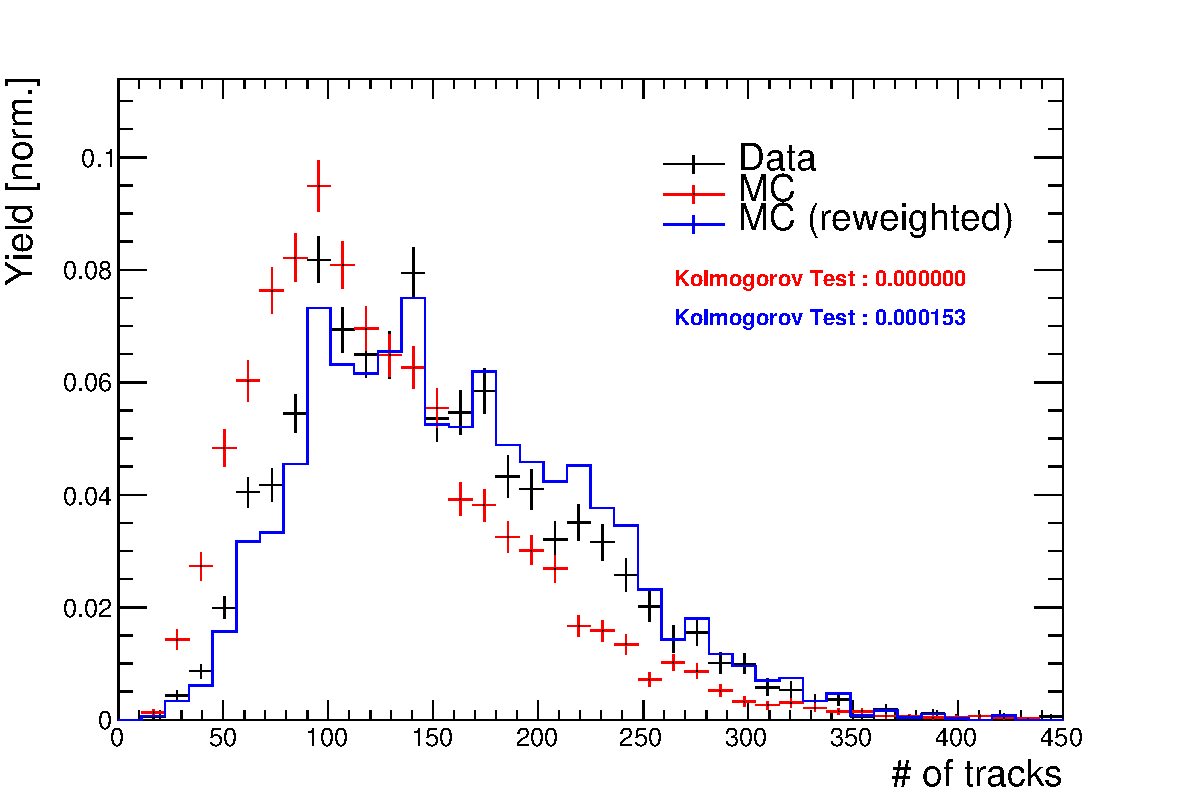
\includegraphics[height=6.cm,width=0.45\textwidth]{figs/MC-v-Data/nTracks.pdf}
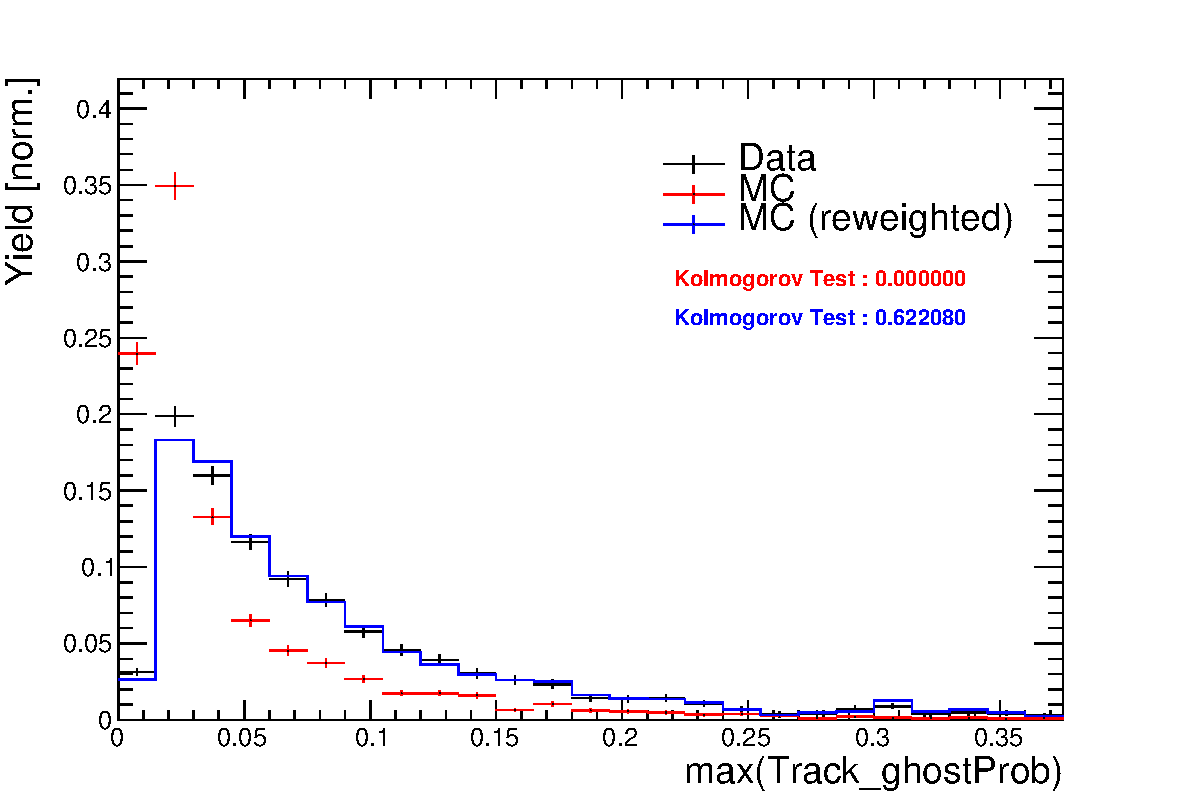
\includegraphics[height=6.cm,width=0.45\textwidth]{figs/MC-v-Data/max_ghostProb.pdf}
\label{fig: reweightingVar}
\caption{Distributions of the (left) number of tracks and the (right) maximum ghost probability over all tracks for data (black), MC (red) and reweighted MC (blue).}
\end{figure}

The following figures show the comparison of all other observables, which were used during the multivariate selection stage.


\begin{figure}[h!]
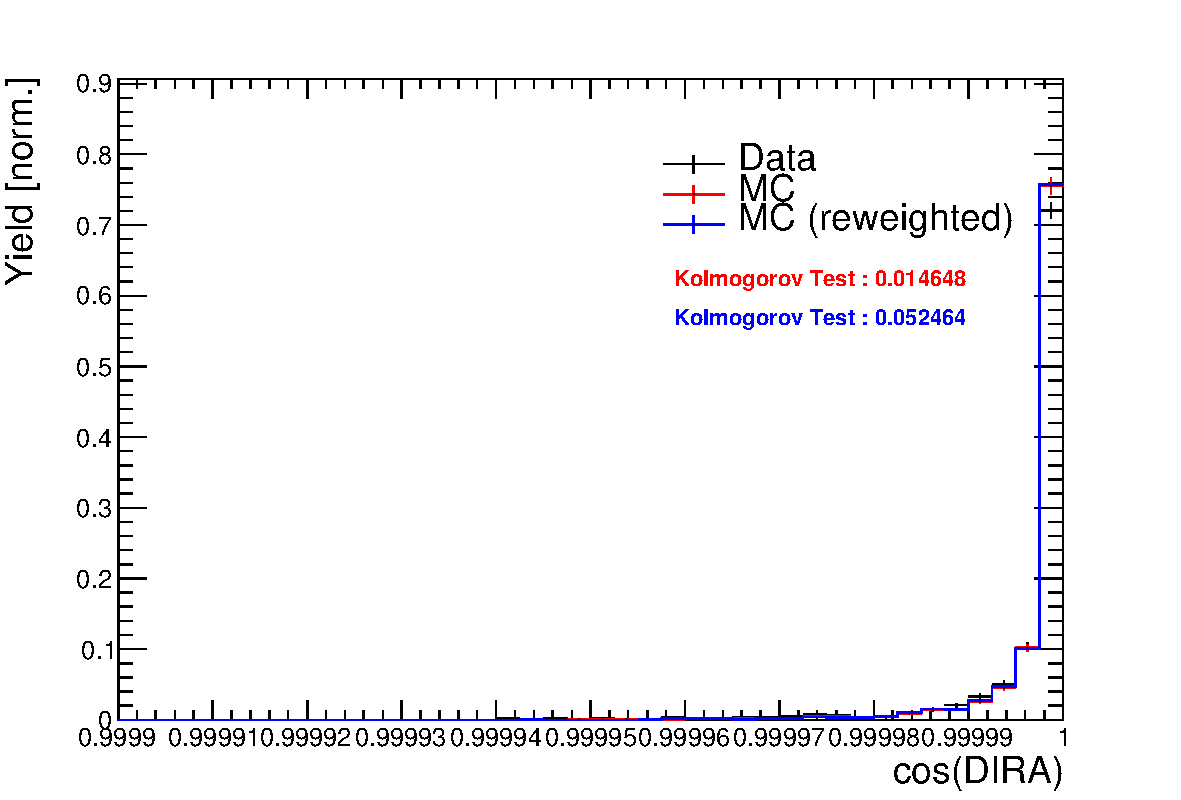
\includegraphics[height=6.cm,width=0.45\textwidth]{figs/MC-v-Data/Bs_DIRA_OWNPV.pdf}
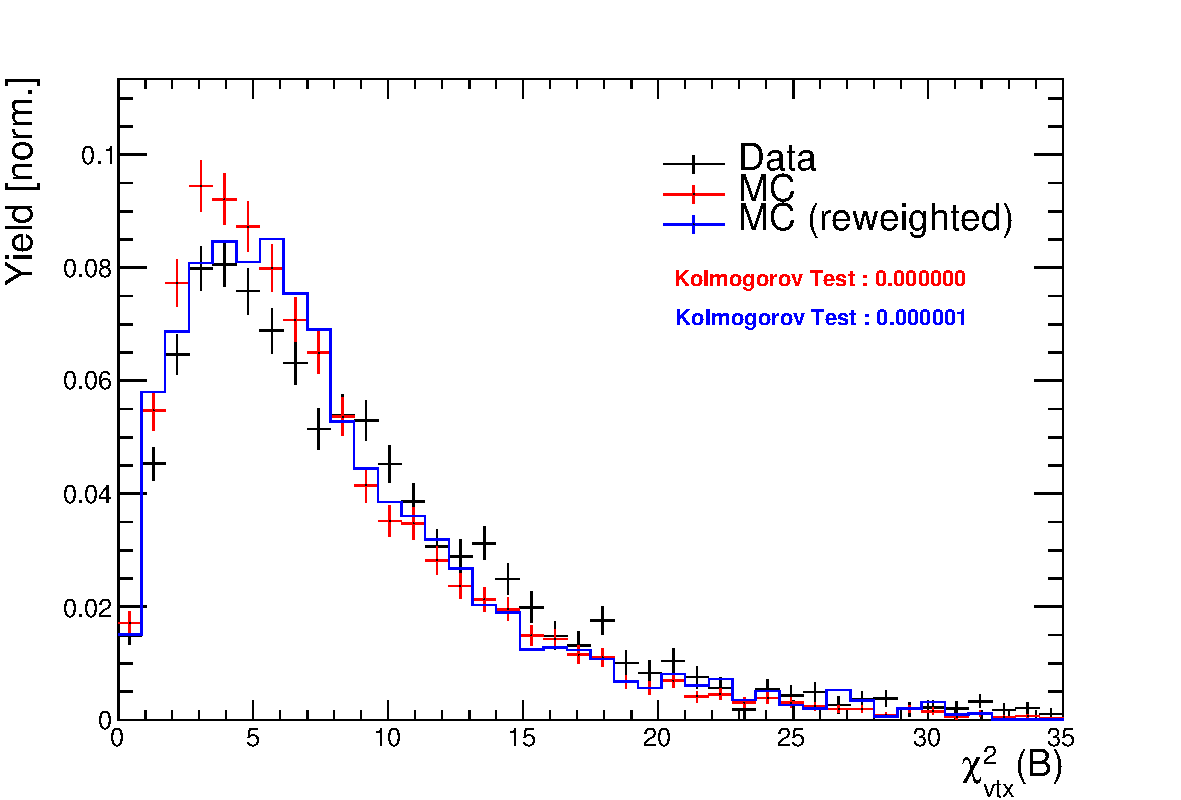
\includegraphics[height=6.cm,width=0.45\textwidth]{figs/MC-v-Data/Bs_ENDVERTEX_CHI2.pdf}\\
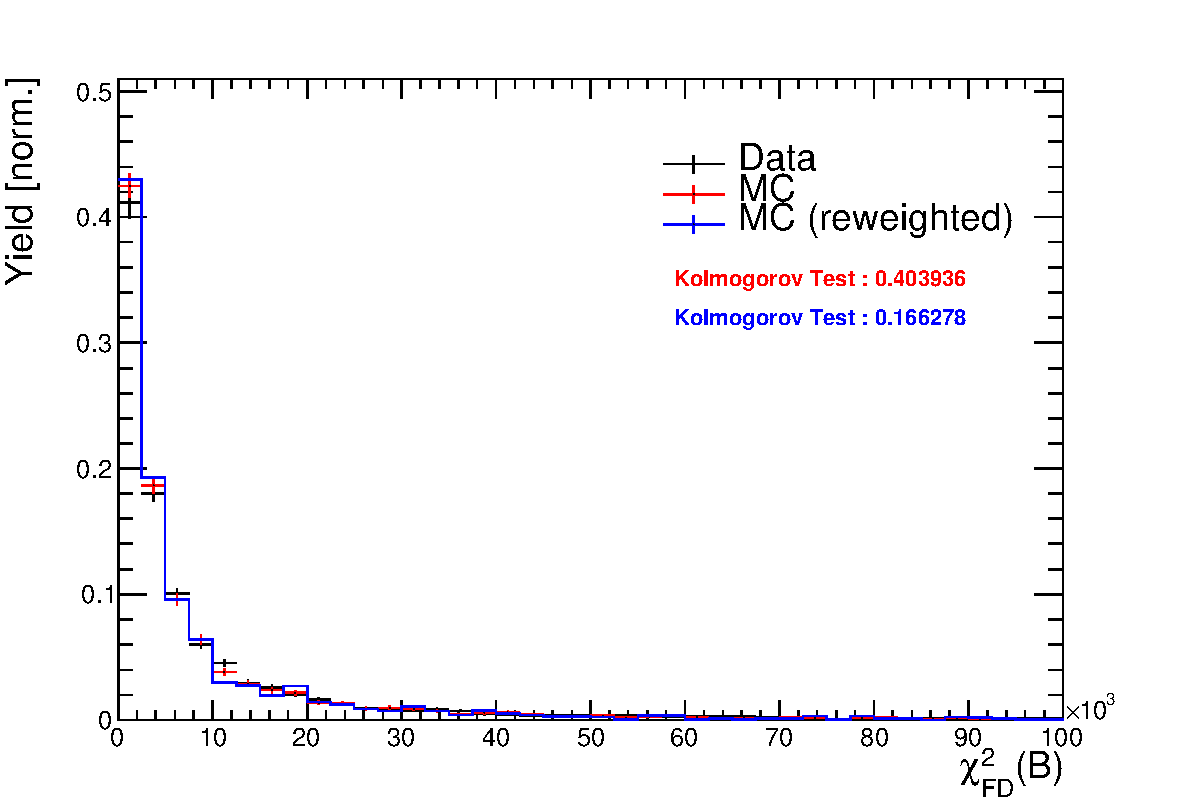
\includegraphics[height=6.cm,width=0.45\textwidth]{figs/MC-v-Data/Bs_FDCHI2_OWNPV.pdf}
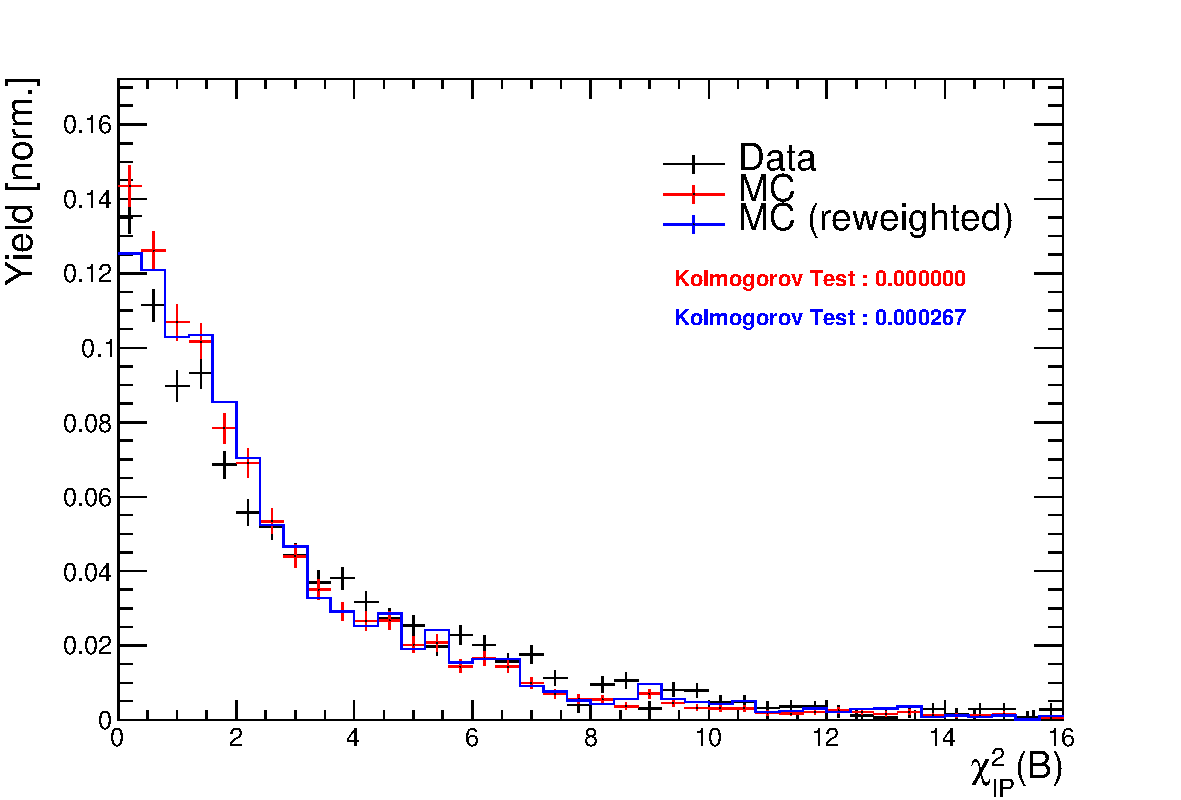
\includegraphics[height=6.cm,width=0.45\textwidth]{figs/MC-v-Data/Bs_IPCHI2_OWNPV.pdf}
\caption{Comparison of data and MC observables, before and after reweighting 1.}
\end{figure}

\begin{figure}[h!]
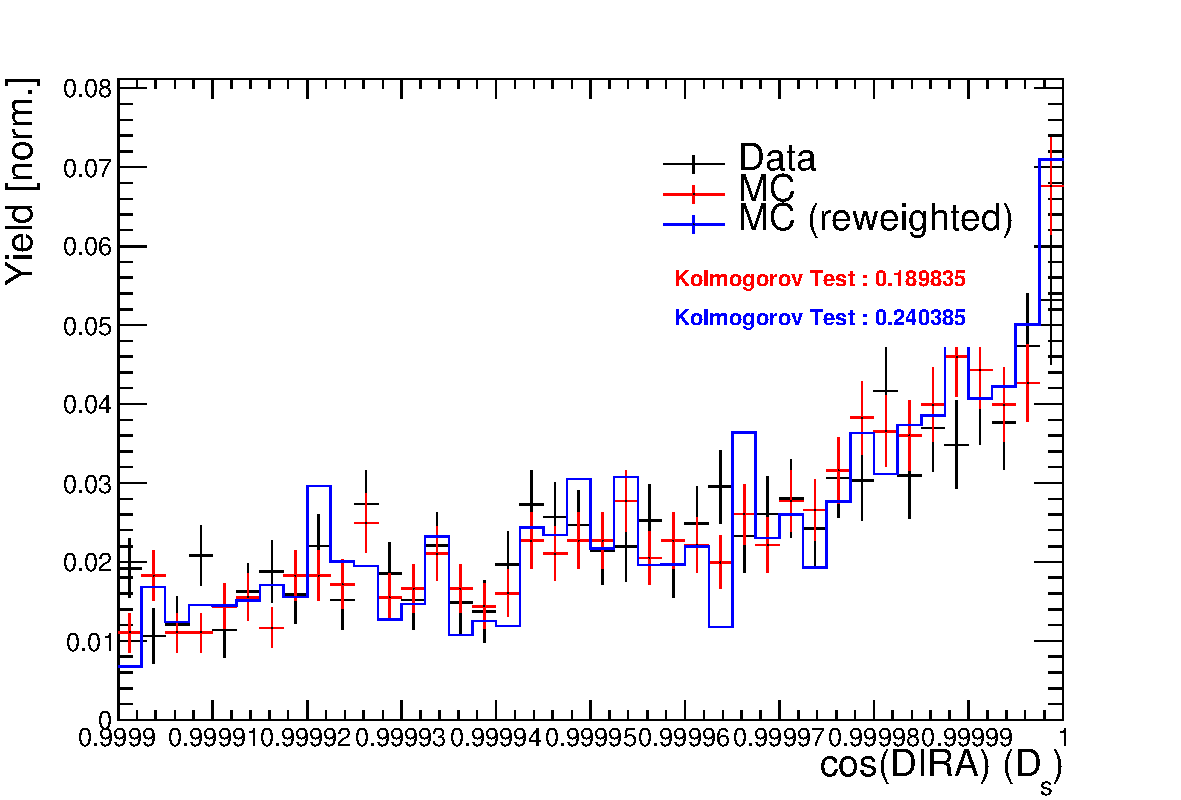
\includegraphics[height=6.cm,width=0.45\textwidth]{figs/MC-v-Data/Ds_DIRA_OWNPV.pdf}
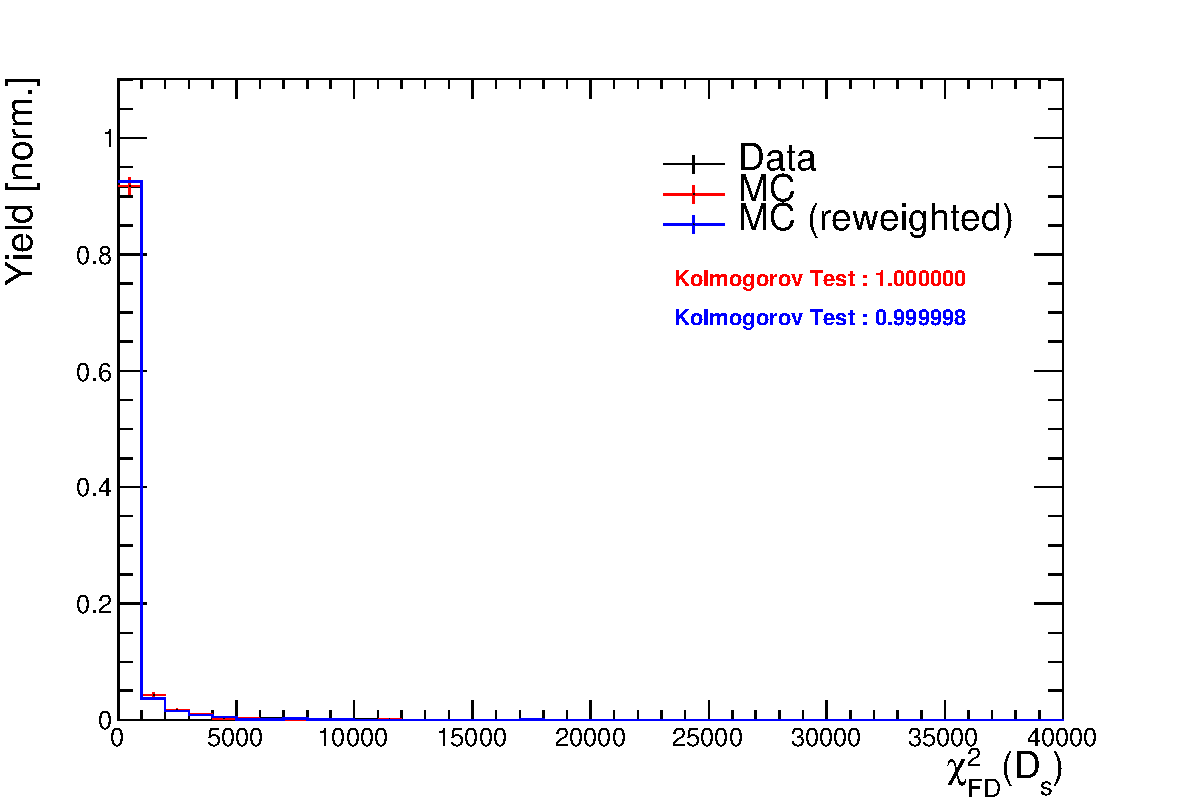
\includegraphics[height=6.cm,width=0.45\textwidth]{figs/MC-v-Data/Ds_FDCHI2_ORIVX.pdf}\\
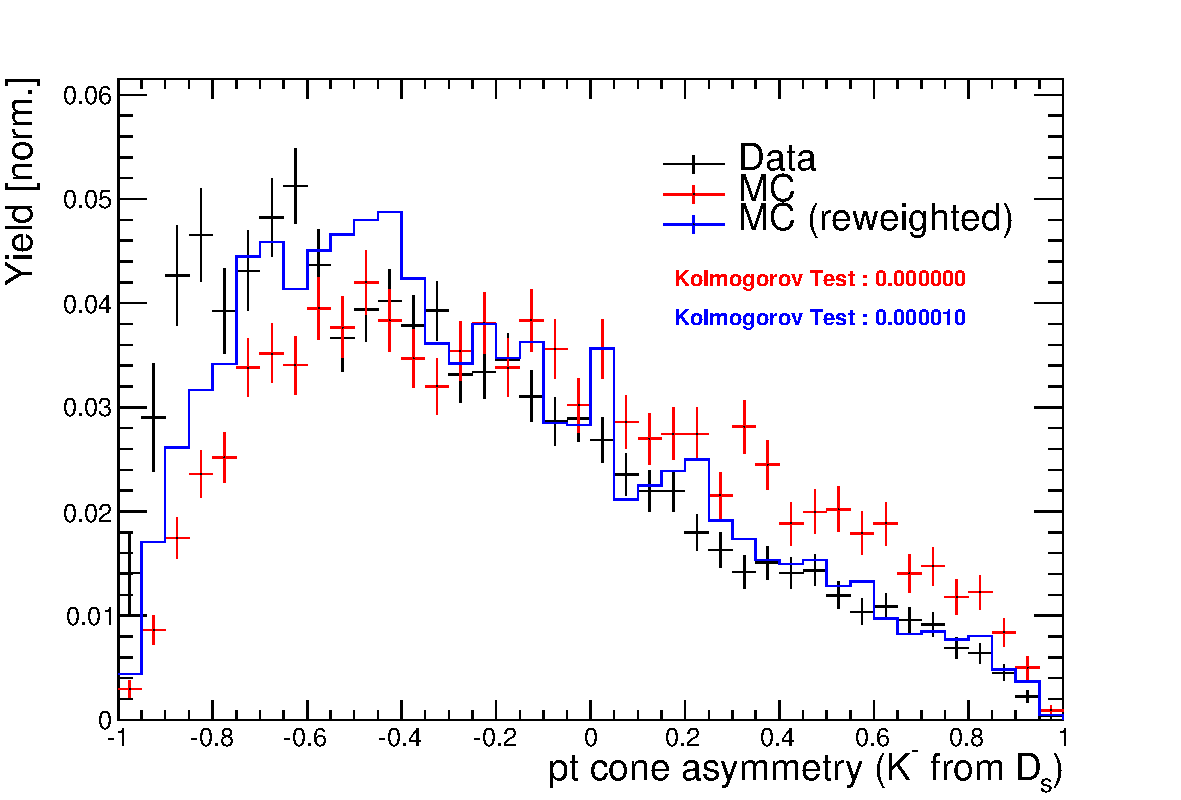
\includegraphics[height=6.cm,width=0.45\textwidth]{figs/MC-v-Data/K_minus_fromDs_ptasy_1_00.pdf}
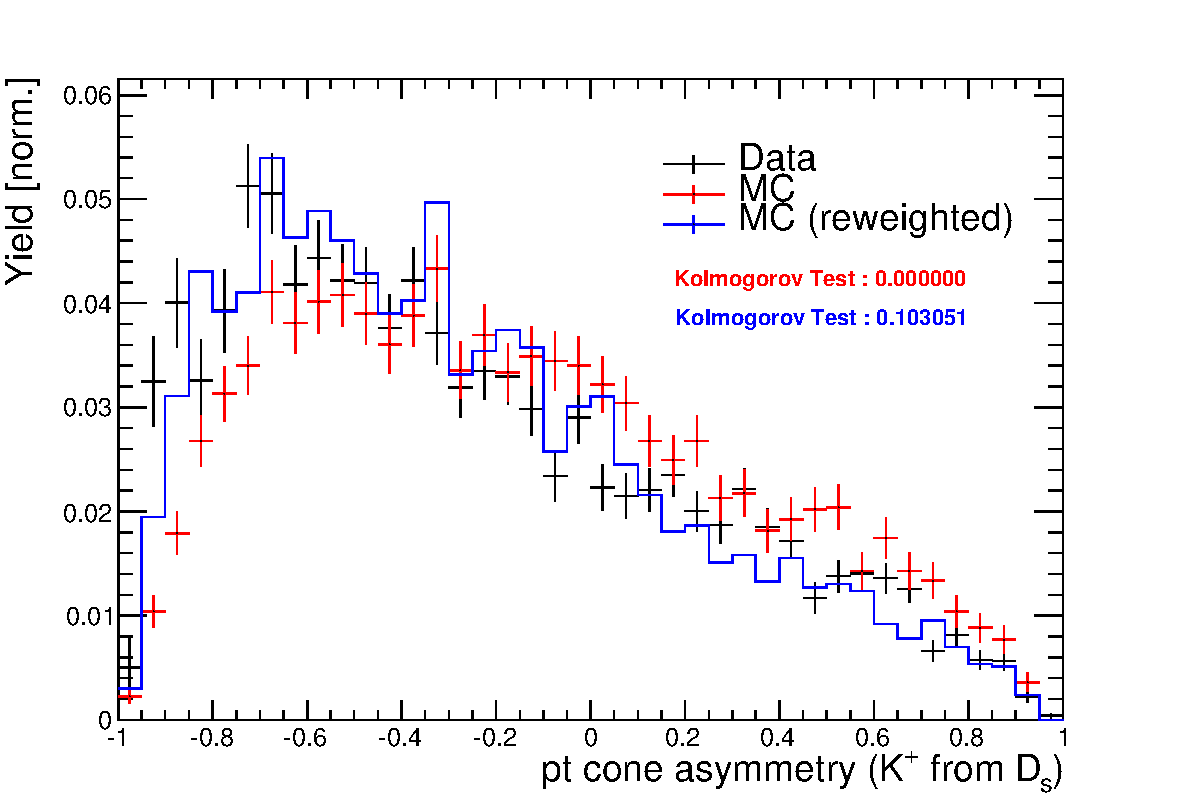
\includegraphics[height=6.cm,width=0.45\textwidth]{figs/MC-v-Data/K_plus_fromDs_ptasy_1_00.pdf}
\caption{Comparison of data and MC observables, before and after reweighting 2.}
\end{figure}

\begin{figure}[h!]
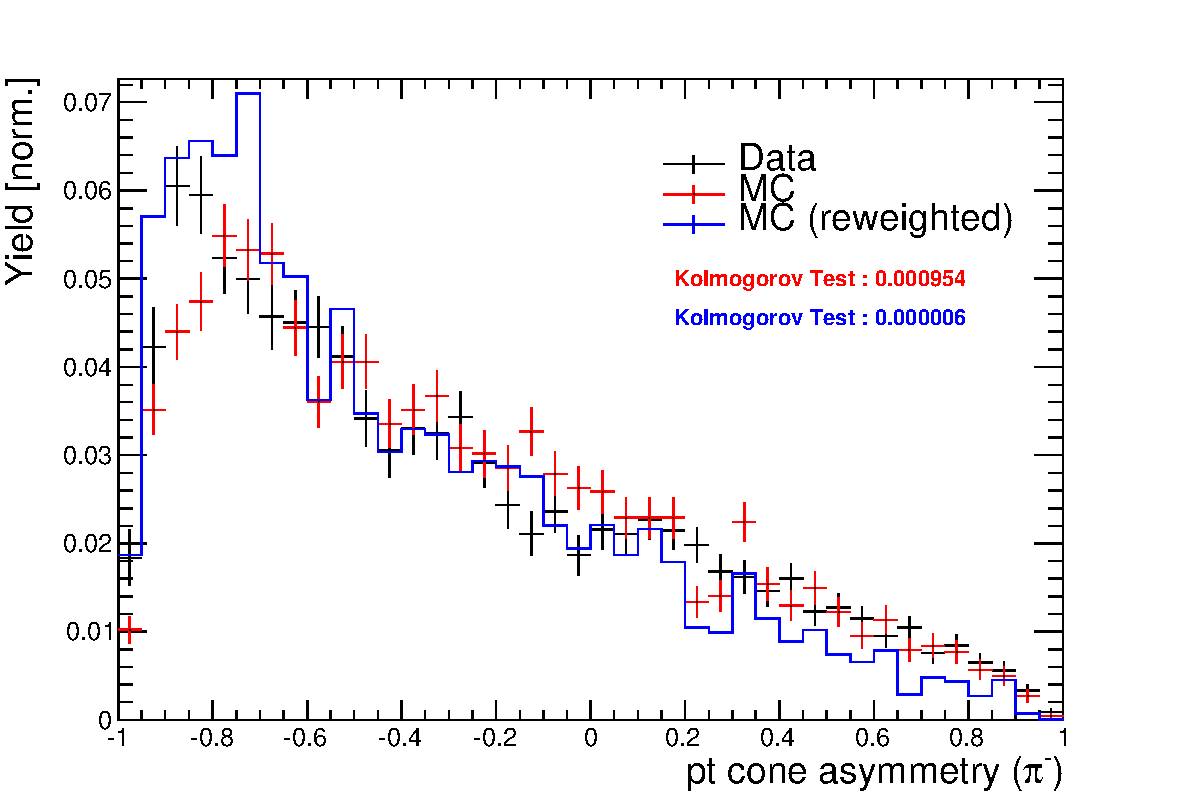
\includegraphics[height=6.cm,width=0.45\textwidth]{figs/MC-v-Data/pi_minus_ptasy_1_00.pdf}
%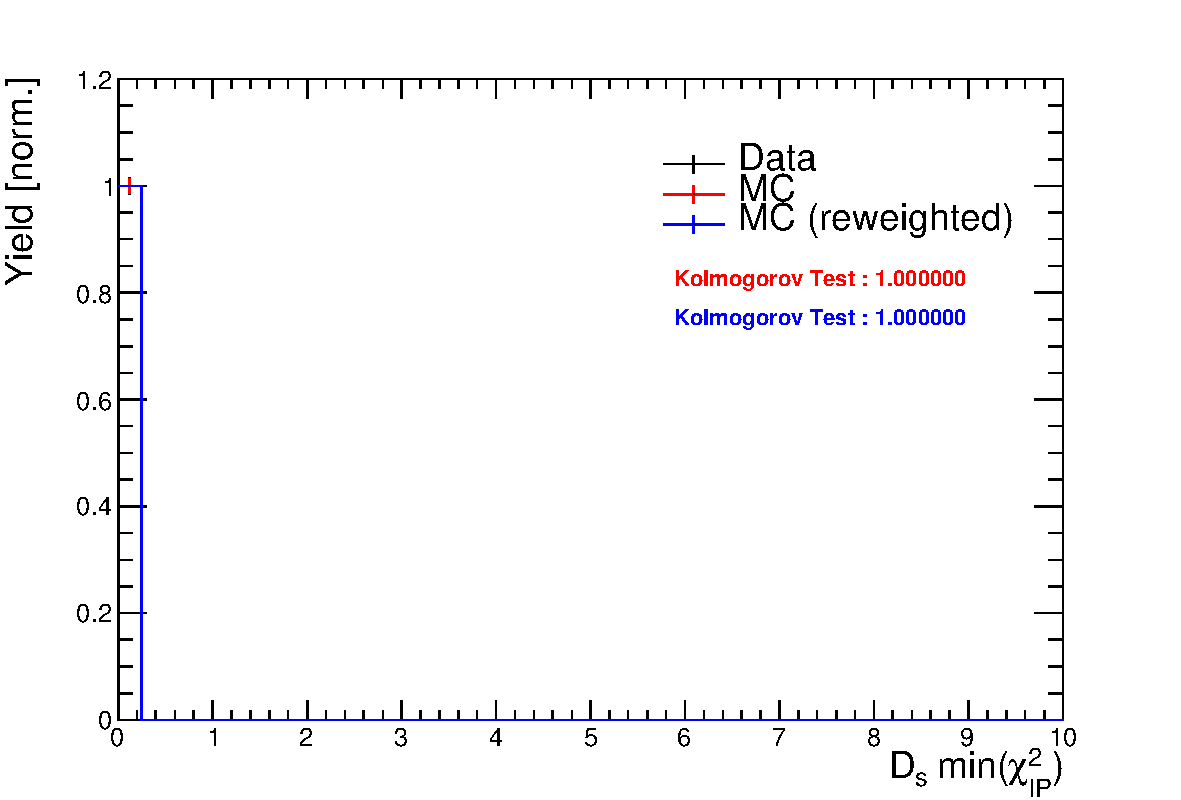
\includegraphics[height=6.cm,width=0.45\textwidth]{figs/MC-v-Data/log_DsDaughters_min_IPCHI2.pdf}\\
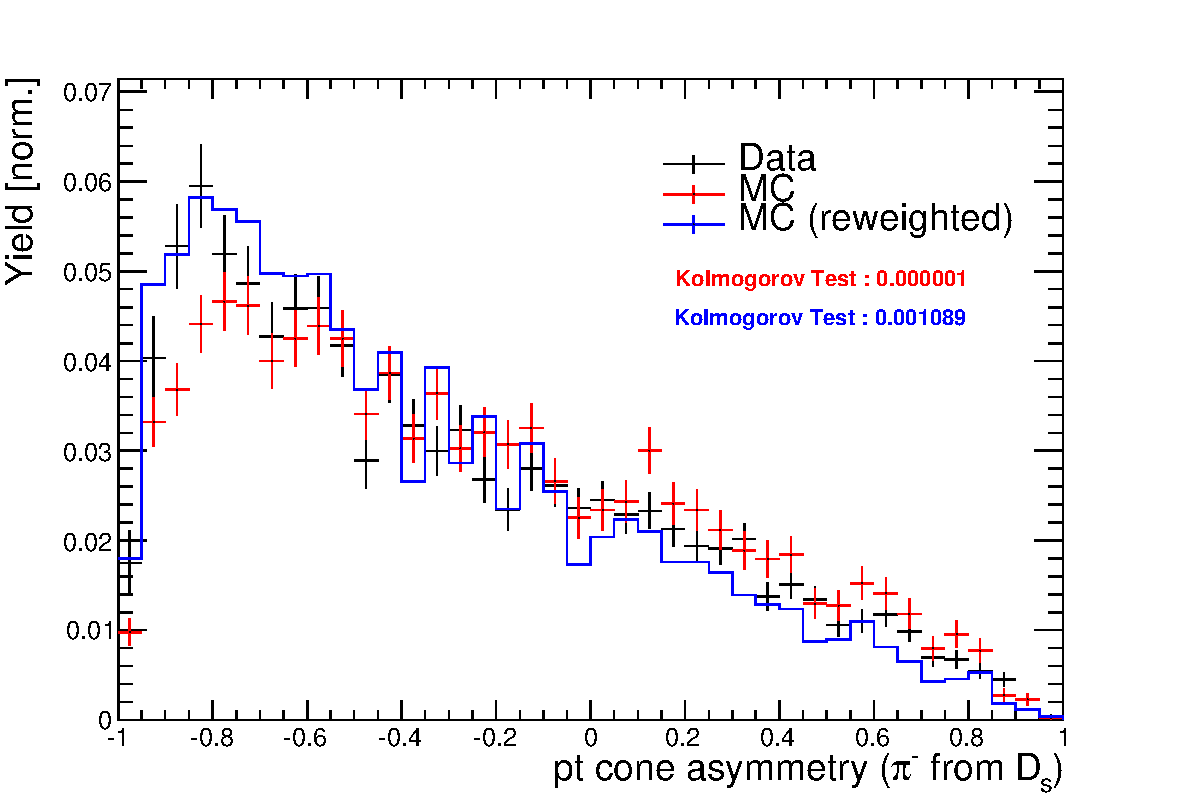
\includegraphics[height=6.cm,width=0.45\textwidth]{figs/MC-v-Data/pi_minus_fromDs_ptasy_1_00.pdf}
\caption{Comparison of data and MC observables, before and after reweighting 3.}
\end{figure}


%\subsection{Toys for normalization fit}
%\label{sec: toysNorm}

%To validate the fit model used to describe the $m(\Ds\pion\pion\pion)$ spectrum, we produce 1000 pseudo samples from our fit pdf and fit them with the same nominal pdf model. \newline
%A pull of a certain fit parameter is defined as

%\begin{equation}
%p = \frac{x - x_{0}}{\Delta x},
%\label{eq: pull}
%\end{equation}  

%where $x$ is the fitted value, $x_{0}$ the generated value and $\Delta x$ the uncertainty on $x$. 
%Given the fit is correctly implemented and unbiased, one expects the distribution of the pulls for every fit parameter to be centered around 0, with a gaussian width of 1.



%\begin{figure}[h]
%\includegraphics[height=6.cm,width=0.45\textwidth]{figs/.pdf}
%\includegraphics[height=6.cm,width=0.45\textwidth]{figs/.pdf}\\
%\includegraphics[height=6.cm,width=0.45\textwidth]{figs/.pdf}
%\includegraphics[height=6.cm,width=0.45\textwidth]{figs/.pdf}
%\caption{Pull distributions for 1000 pseudo experiments, using the fit model for the normalization fit. Part 1.}
%\end{figure}


\FloatBarrier
